\newpage
\subsection{Управление продажами}
\label{bp:SalesManagment}


Менеджер  ведёт общий план по производству. 
Клиент высылает менеджеру заявку на изготовление продукции. 
Типовой формы заявки не выявлено.
Заявка высылается в произвольном виде по емайл, через мессенджеры. 



При поступлении заявки на изготовление продукции Менеджер в системе 1С:УПП формирует заявки покупателя (рис. \ref{pic:d11}). Менеджер создает при необходимости документ ''Счет'' на оплату из формы \ref{pic:d11}. 
Менеджер при необходимости создает в системе 1С:УПП новый договор.
Дата отгрузки в заявке является желаемой датой покупателя. 

В системе 1С:УПП есть модуль объёмно календарного планирования (рис. \ref{pic:d10}), в котором менеджер может запланировать выполнение заказа клиента.
Менеджер создаёт заказ на производство в системе 1С:УПП.
 Менеджер утверждает  в системе 1С:УПП заказ на производство (форма (рис. \ref{pic:d10}).

Менеджер проводит заказ в системе 1С:УПП.

Каждое утро в 9-00 бухгалтер в системе 1С:УПП вносит выписки из банка.
Менеджеры видят информацию по оплате покупателей в системе 1С:УПП. Каждый менеджер при необходимости обзванивает должников. 

Отдел планирования может выгружать заказы из системы 1С:УПП для оперативного планирования.

% % Менеджер заказывает заготовки точно под требуемый объем продукции и в нужный размер под готовую продукцию.
% На каждый заказ производства есть только одна заготовка.
% %Менеджер создает заказ на сторону только исходя из объема заказа на производство.
% Заказ заготовок создается точно по объему готовой продукции без дополнительных заготовок на пусконаладку. Отклонения в объеме готовой продукции прописаны в спецификациях к договору.
% % Дополнительные заготовки на пусконаладку не закупаются.
% Каждый МСЗ на основании заказа покупателя формирует заказ заготовок кратно транспортной единице (Фура). На предприятии заказывают до 12 фур в неделю заготовок. МСЗ считает загрузку транспорта вручную. Отгрузка продукции и заготовок осуществляется строго на паллетах.

% Каждое утро в 9-00 бухгалтер присылает выписки из банка. Менеджеры видят информацию по оплате покупателей в системе 1С:УНФ. Каждый менеджер при необходимости обзванивает должников. 


% Коммерческий директор ведет анализ продаж по событиям в системе 1С:УНФ.

% Покупатель может прислать дополнительную заявку кроме месячного плана.
%Все поступающие заявки менеджер фиксируют в файле “План” (см. \ref{pic:monthplan}).

%
%Менеджер может разбить заявку покупателя на части с учётом загрузки в транспорт. 

%Менеджер печатает заявку покупателя по форме \ref{pic:SalesOrder}. В форме \ref{pic:SalesOrder} есть три экземпляра: один остается у менеджера, один передается на планирование переработки, один передается на планирование раскроя.   


%Заявку распечатанную в формате MS Excel менеджер передает экономисту для проверки задолженности. Экономист ставит свой штамп на бланке при одобрении заявки. Подписанную заявку менеджер передает в плановый отдел (плановик коммерческом отделе). Экономист может запретить запуск по контролю оплаты, плохим условиям по арбитражу у контрагента. Заявка может быть не одобрена при отсутствии подписанного договора.



%
%
%\begin{figure}
%\begin{center}
%  \includegraphics[width=\linewidth, height=0.94\textheight, keepaspectratio]{Pics/prodline_loading.jpg}
%\end{center}
%  \caption{Отчет по загруженности линий.}
%  \label{pic:prodline_loading}
%\end{figure}
%\clearpage
%%

%%
%\begin{figure}
%\begin{center}
%  \includegraphics[height=0.94\textheight, keepaspectratio]{Pics/SalesOrder.jpg}
%\end{center}
%  \caption{Форма заявки покупателя}
%  \label{pic:SalesOrder}
%\end{figure}
%\clearpage


%%
%%
%%\begin{figure}
%%\begin{center}
%%\ifnum\pdfoutput=0
%%  \includegraphics[40,0][366,292]{Pics/CostRequest.png}
%%\else 
%%  \includegraphics[height=0.94\textheight, keepaspectratio]{Pics/CostRequest.jpg}
%%\fi
%%\end{center}
%%  \caption{Форма опросного листа покупателя}
%%  \label{pic:CostRequest}
%%\end{figure}
%%\clearpage
%%
%При поступлении заявки от покупателя по существующему изделию менеджер отдела продаж принимает заявку покупателя. Единого реестра заявок  не обнаружено. 
%Менеджеры отдела продаж проверяют оплату от покупателя по условиям договора.  
%Дата отгрузки это желаемая дата клиента. Дата производства по договору это дата отгрузки минус пять дней.
%Менеджер формирует заявку в формате Word и/или в программе 1С: ERP, распечатывает, подписывает, сканирует и формате pdf выкладывает на сервер для отдела планирования. 
%
%Небольшие разовые заказы менеджер по сопровождению сразу заносит в программу 1С, распечатывает, подписывает, сканирует формат PDF и выкладывает на сервер для планировщика.
%
%Появление файла сканированного в сетевом каталоге означает запуск производства заказов производством. 
%
%% 
%%При положительном решении по оплате менеджер ОСЛ создает заказ производственный. 
%%Каждый менеджер ОСЛ фиксирует заявку в портфеле заказов (см. рис. \ref{pic:WorkOrderList}).
%%
%%
%%
%%
%%\begin{figure}
%%\begin{center}
%%  \includegraphics[height=0.94\textheight, keepaspectratio]{Pics/WorkOrderList.jpg}
%%\end{center}
%%  \caption{Форма портфеля заказов по менеджеру отдела сбыта и логистики}
%%  \label{pic:WorkOrderList}
%%\end{figure}
%%\clearpage
%
%
%
%%На момент обследования любое изделие из картона на предприятии рассматривается как новое изделие. Для запуска производства менеджером отдела сбыта начинается выполнение процесса "Подготовка производства" (см. процесс \ref{BP_Prepare}).
%%
%%В систему 1С УПП менеджеры при необходимости заводят новые позиции в справочник "Контрагенты".
%%На предприятии существует стандартный прайс на продукцию (см. \ref{pic:Price}).
%%Позиции в прайсе представляют стандартные изделия, изготавливаемые на склад без заказчика.
%%
%%В отдел сбыта к менеджерам поступает заявка от заказчиков. Типовой формы заказа не существует. 
%%На основании принятой заявки от заказчика менеджер должен определить цену продажи.
%%На момент обследования любое изделие из картона на предприятии рассматривается как новое изделие. 
%%В системе 1С менеджер создает документ ''Заказ в производство'' и из программы печатает форму служебной записки (см. рис. \ref{pic:WorkOrder}).
%%Менеджер вручную заполняет требования к изделию в бланке (см. рис. \ref{pic:CostRequest}) и передает форму в отдел ТКО (см. процесс \ref{BP_Prepare}).
%%Для запуска производства менеджером отдела сбыта начинается выполнение процесса "Подготовка производства" (см. процесс \ref{BP_Prepare}).
%%
%%Одним из результатом процесса ''Подготовка производства'' является цена продажи готового изделия. Рассчитанная в ходе указанного процесса цена фиксируется в договоре на производство, указывается в счетах на оплату. Менеджер отдела сбыта формирует в системе 1С УПП форму договора с заказчикоми и счет на оплату.
%%При согласовании изделий и их цены менеджер также должен согласовать условия доставки. Доставка может осуществляться как собстсвенными силами заказчика, так и за счет исполнителя. Во втором случае условия доставки и стоимость прописываются в условиях договора и фиксируются в счете на оплату. 
%%
%%Контроль оплаты производится менеджерами на основании банковской выписки из клиент-банка или по данным бухгалтерии в системе 1С УПП. На момент обследования менеджеры пользуются банковской выпиской из программ клиент-банка.
%%
%%После подтверждения поступления оплаты менеджеры отдела продаж запускают производство. 
%%Служебная записка передается в ТКО для изготовления РРК. Комплект из служебной записки и РРК передается начальнику производства для запуска производства, запуская процесс ''Оперативное планирование'' (см. \ref{bp:OperPlan}).
%%


% \begin{figure}
% \begin{center}
%  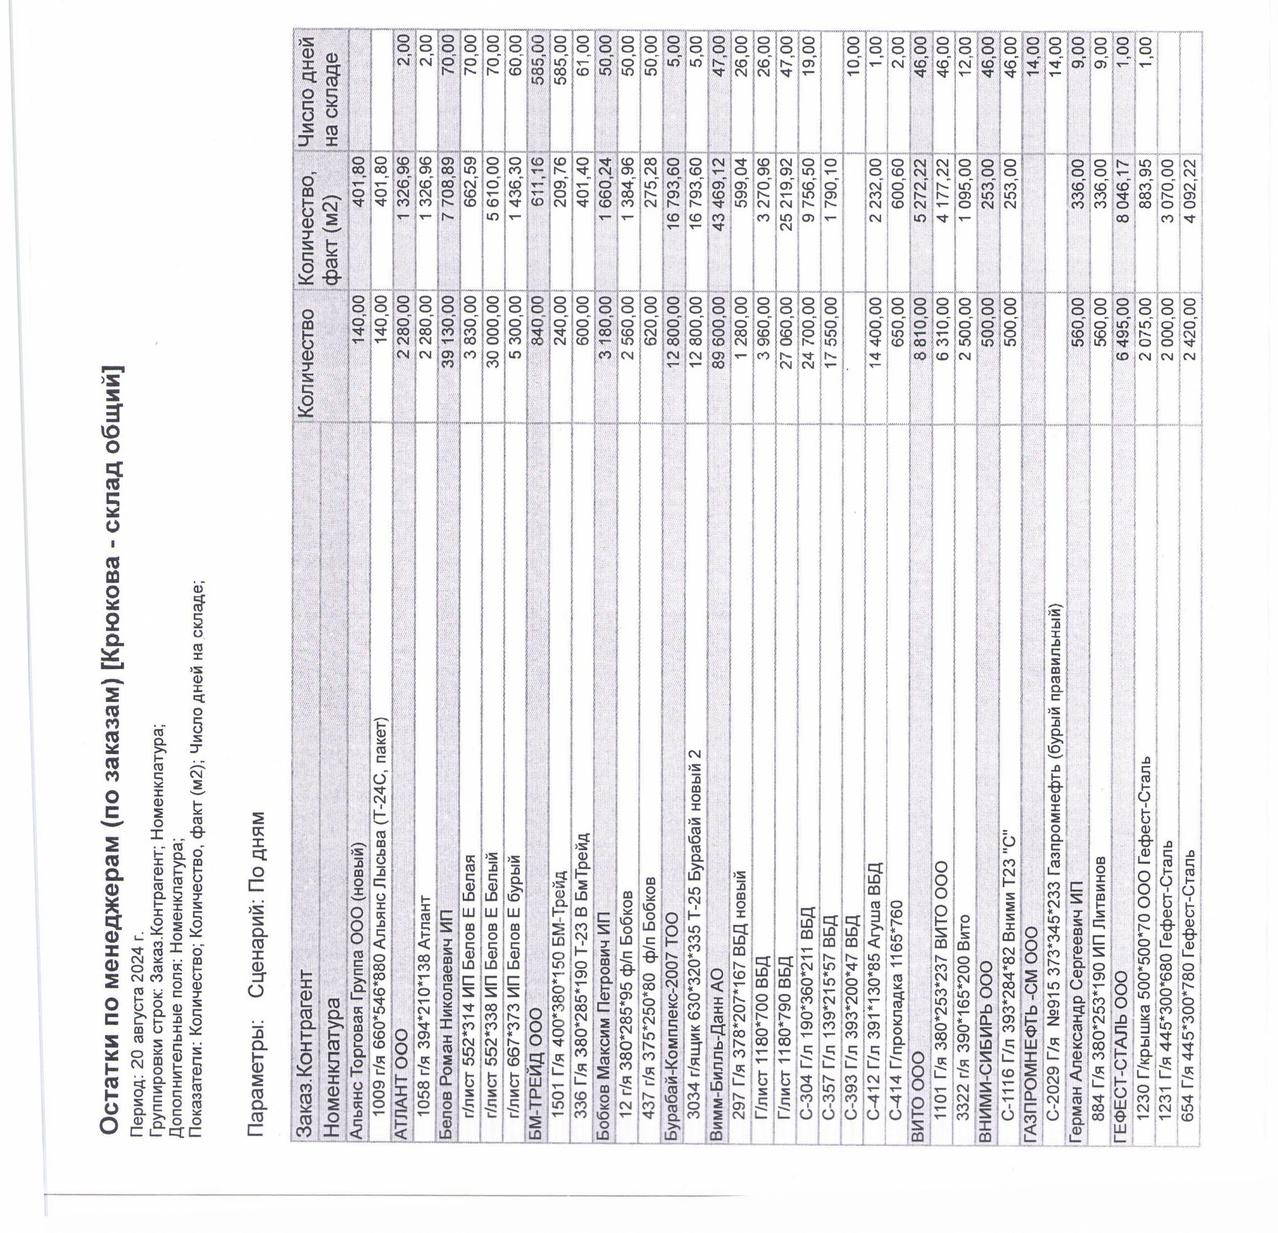
\includegraphics[height=0.4\textheight,   keepaspectratio]{Pics/d14.jpg}
% \end{center}
%  \caption{Форма заказа покупателя в системе 1С: УНФ}
%  \label{pic:d14}
% \end{figure}
% \clearpage


\begin{figure}
\begin{center}
 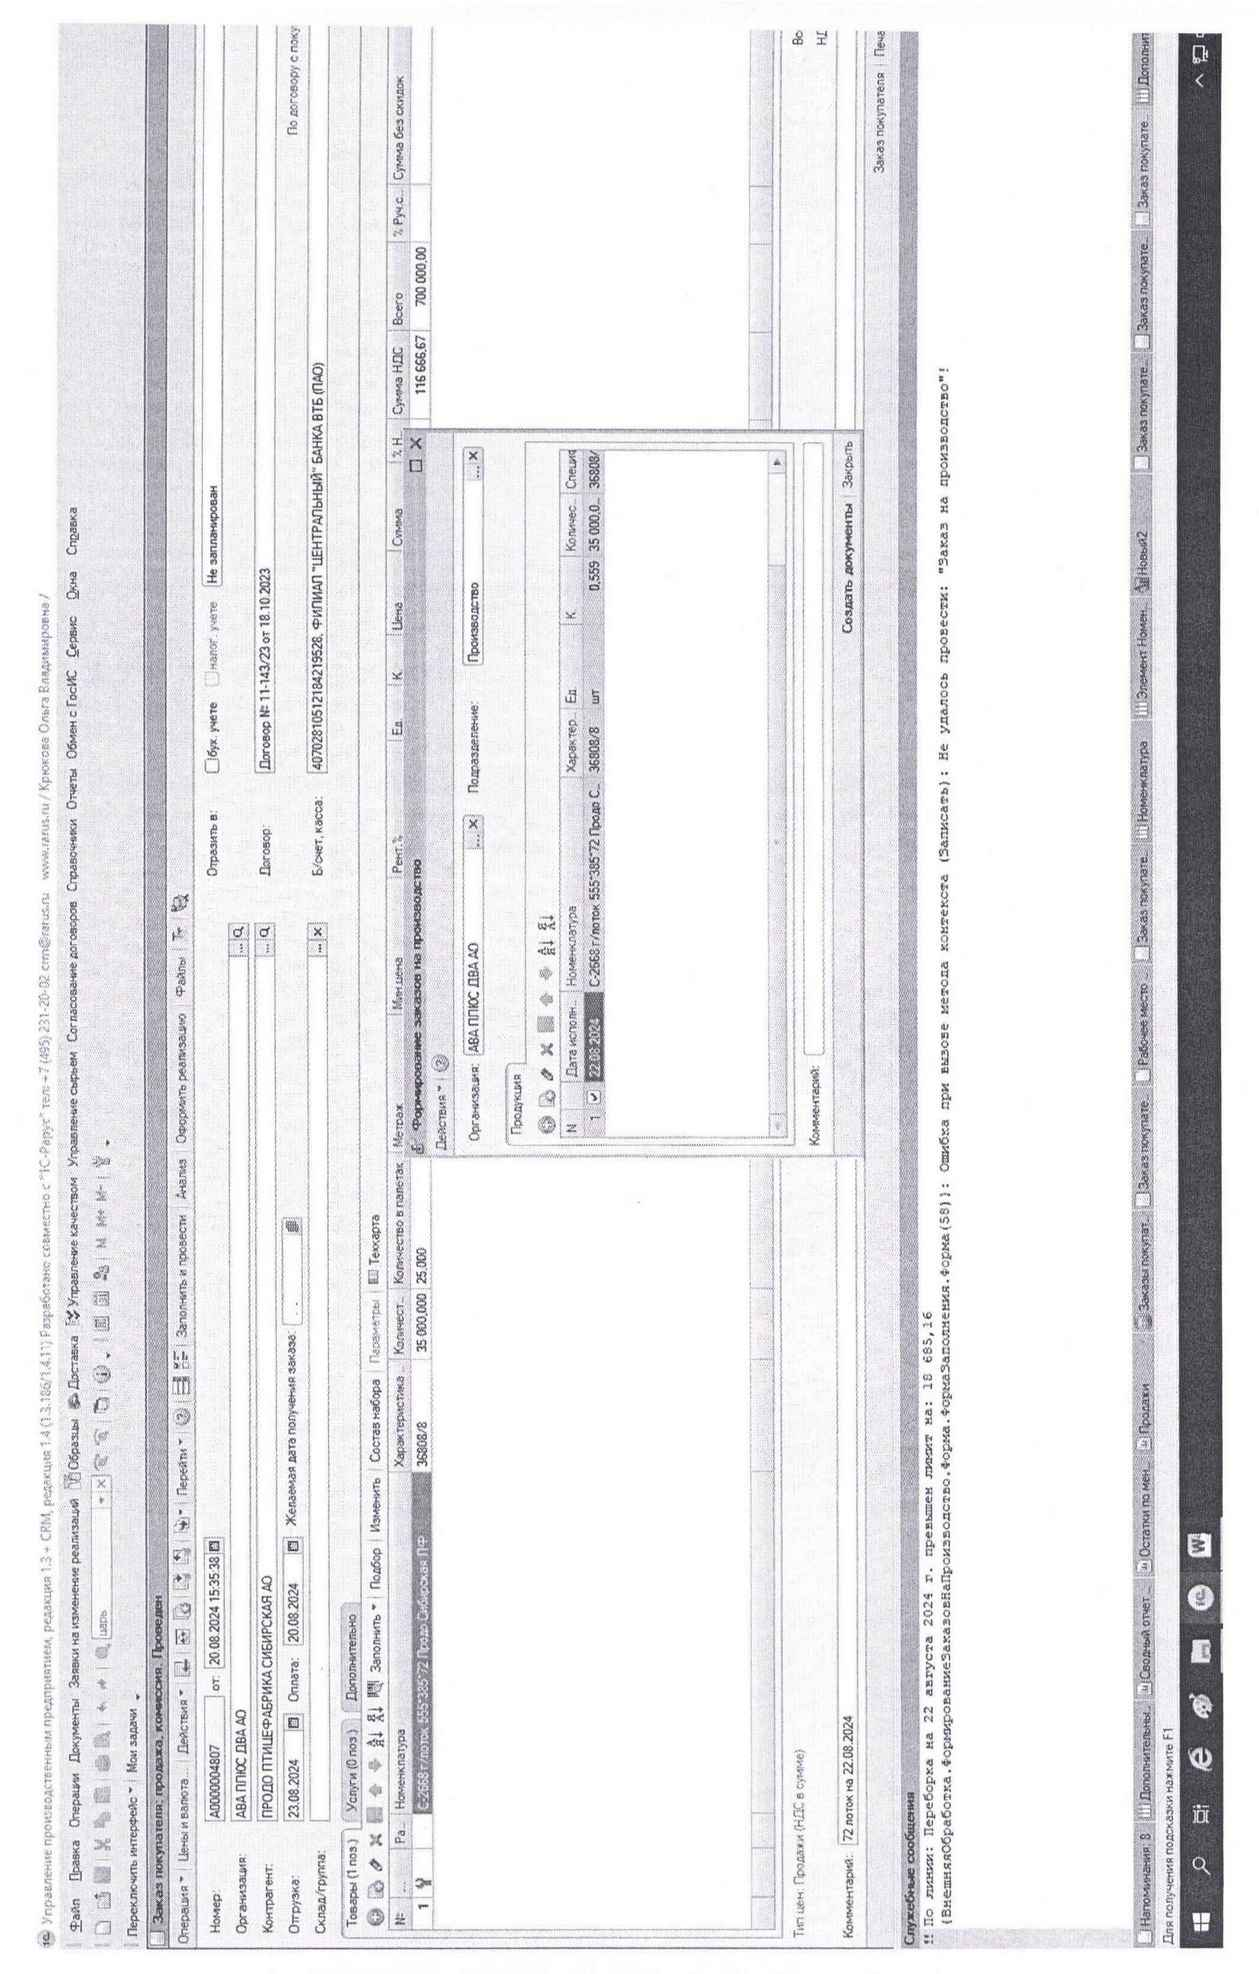
\includegraphics[height=0.8\textheight, keepaspectratio]{Pics/d11.jpg}
\end{center}
 \caption{Форма заявки покупателя в системе 1С:УПП}
 \label{pic:d11}
\end{figure}

\begin{figure}
\begin{center}
 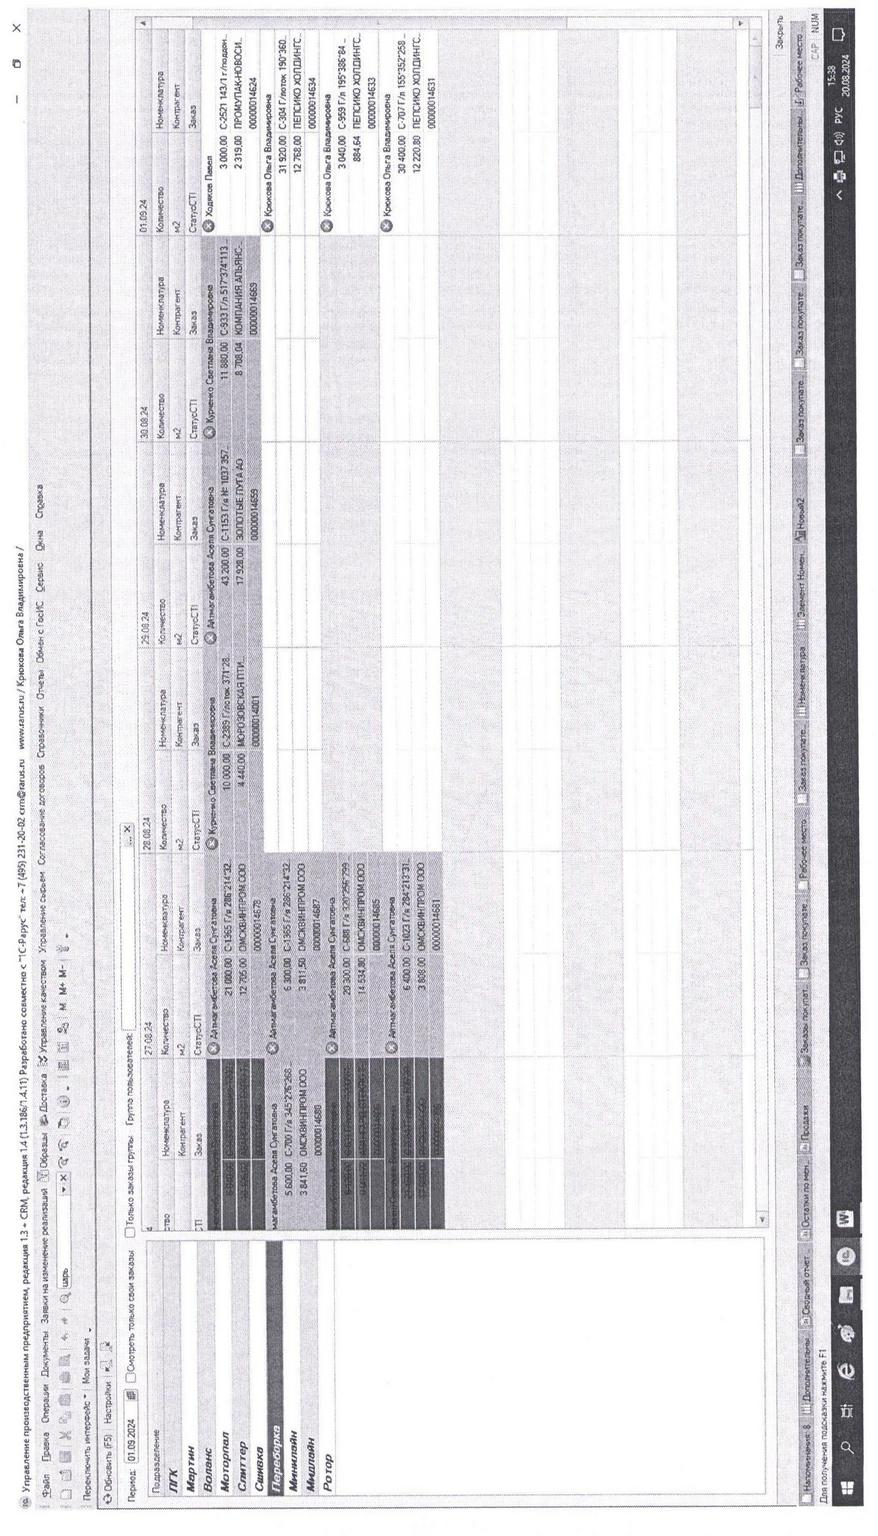
\includegraphics[height=0.8\textheight, keepaspectratio]{Pics/d10.jpg}
\end{center}
 \caption{Форма объёмно календарного планирования}
 \label{pic:d10}
\end{figure}





\clearpage
\ifx \notincludehead\undefined
\normalsize
\end{document}
\fi